\documentclass[tikz,border=10pt]{standalone}
\usetikzlibrary{arrows.meta,positioning,fit,backgrounds}

\definecolor{datablue}{HTML}{DCEEFF}
\definecolor{processgreen}{HTML}{DDF2E1}
\definecolor{trainpurple}{HTML}{E7DDF5}
\definecolor{validationyellow}{HTML}{FFF0C7}
\definecolor{policyorange}{HTML}{FAD9B8}
\definecolor{testblue}{HTML}{D5E8F6}

\tikzset{
  stage/.style={
    draw=black!75,
    rounded corners=3pt,
    minimum width=29mm,
    minimum height=14mm,
    align=center,
    font=\small,
    line width=.7pt
  },
  flow/.style={
    -{Latex[length=2.4mm]},
    draw=black!75,
    line width=.8pt
  },
  splitlabel/.style={font=\scriptsize, text=black!60, align=center},
  phase/.style={draw=black!40, rounded corners=4pt, dashed, inner sep=5pt}
}

\begin{document}
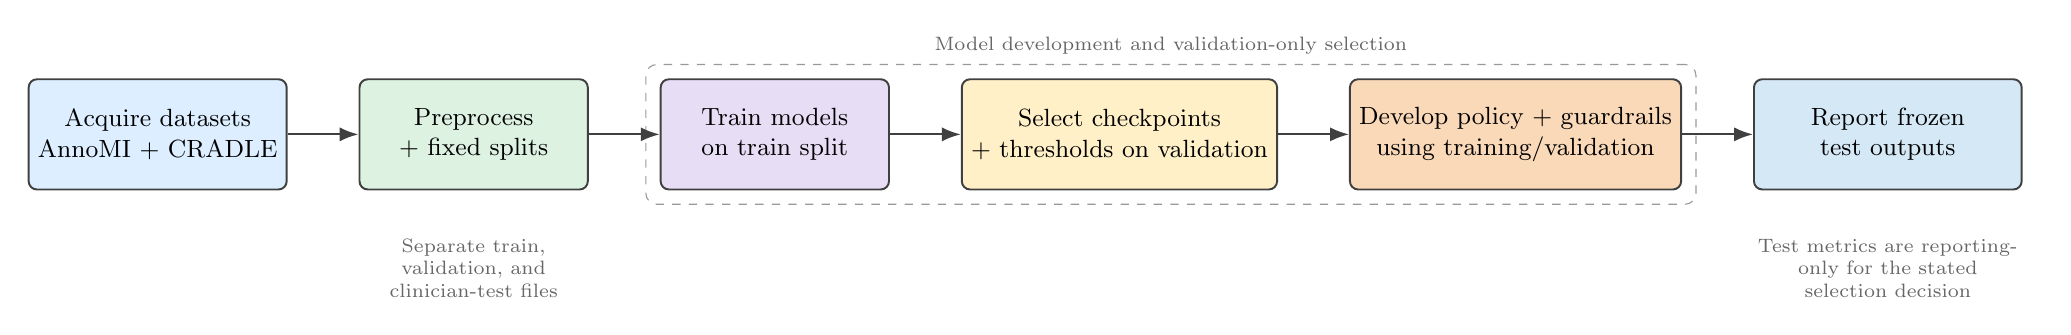
\begin{tikzpicture}[node distance=9mm]

\node[stage, fill=datablue] (acquire)
  {Acquire datasets\\AnnoMI + CRADLE};
\node[stage, fill=processgreen, right=of acquire] (preprocess)
  {Preprocess\\+ fixed splits};
\node[stage, fill=trainpurple, right=of preprocess] (train)
  {Train models\\on train split};
\node[stage, fill=validationyellow, right=of train, minimum width=36mm] (select)
  {Select checkpoints\\+ thresholds on validation};
\node[stage, fill=policyorange, right=of select, minimum width=39mm] (policy)
  {Develop policy + guardrails\\using training/validation};
\node[stage, fill=testblue, right=of policy, minimum width=34mm] (test)
  {Report frozen\\test outputs};

\draw[flow] (acquire) -- (preprocess);
\draw[flow] (preprocess) -- (train);
\draw[flow] (train) -- (select);
\draw[flow] (select) -- (policy);
\draw[flow] (policy) -- (test);

\begin{scope}[on background layer]
  \node[phase, fit=(train)(select)(policy),
    label={[splitlabel]above:Model development and validation-only selection}] {};
\end{scope}

\node[splitlabel, below=5mm of preprocess, text width=31mm]
  {Separate train, validation, and clinician-test files};
\node[splitlabel, below=5mm of test, text width=37mm]
  {Test metrics are reporting-only for the stated selection decision};

\end{tikzpicture}
\end{document}

